\chapter{Android Malware Evaluation Detection and Analysis}
\label{sec:architecture}

\section{Goals}
Android Malware Evaluation Detection and Analysis (AndroMEDA) is designed to complement existing Android security extensions\citep{All security extensions}. The goal in building AndroMEDA was the minimal amount of changes to the Android system, to extract sufficient information. Portability was important, as code that is easier to port can be more easily adopted. Along with the goal of being lightweight and fast, this further forced the extension to be as simple as possible. The framework aimed to be as independent of hardware as possible, as to work on any device - smartphone, tablet, TV, or future devices like Google Glass. This meant as little changes to the low-level drivers and kernel as possible.

Functionally speaking, the main goals of the framework are to better understand how apps behave, what PII and capabilities they access, and to provide the user with the information necessary to quickly evaluate an app's actions in relation to it's UAA. Logging sensitive events, and finding strategic opportunities to expose them to the user, giving the user actions to perform in reaction, is a key step in mitigating Malware, especially Info Theft Malware, on Android. Unfortunately, as discussed in Chapter \ref{sec:permissionrejection}, Android does not log these sensitive events natively, motivating this framework. Ultimately, it's expected that a framework like this will not eliminate malware on android, but rather be part of a larger holistic system.

As a base for our framework, we chose CyanogenMod\citep{cyanogenmod}. CyanogenMod is a 3rd party open source Android distribution created by volunteers. It provides firmware for a wide variety of Android devices, and it's user-base are people seeking to replace their stock OS. This makes it an ideal candidate to fork our framework from - our changes can therefore be incorporated into the over 4.1m+ installs of CyanogenMod\citep{cyanogenmodstats}.

\section{AndroMEDA Architecture}
Android, as an open source project, is hosted at \url{source.android.com}\citep{androidsource}, as a series of \textit{git} repositories managed by a meta-script called \textit{repo}. It's source tree is organized by project type, ``frameworks'', ``external'' and ``libcore'' being the top level folders we focus on. ``frameworks'' contains all of the java, c++, c, assembly, and other code that compose the core framework that runs on top of the main libraries. ``libcore'' and parts of ``external'' comprise the main libraries. The bulk of the code lies in ``frameworks/base''.

%maybe add more?

\begin{figure}[t]
\begin{center}
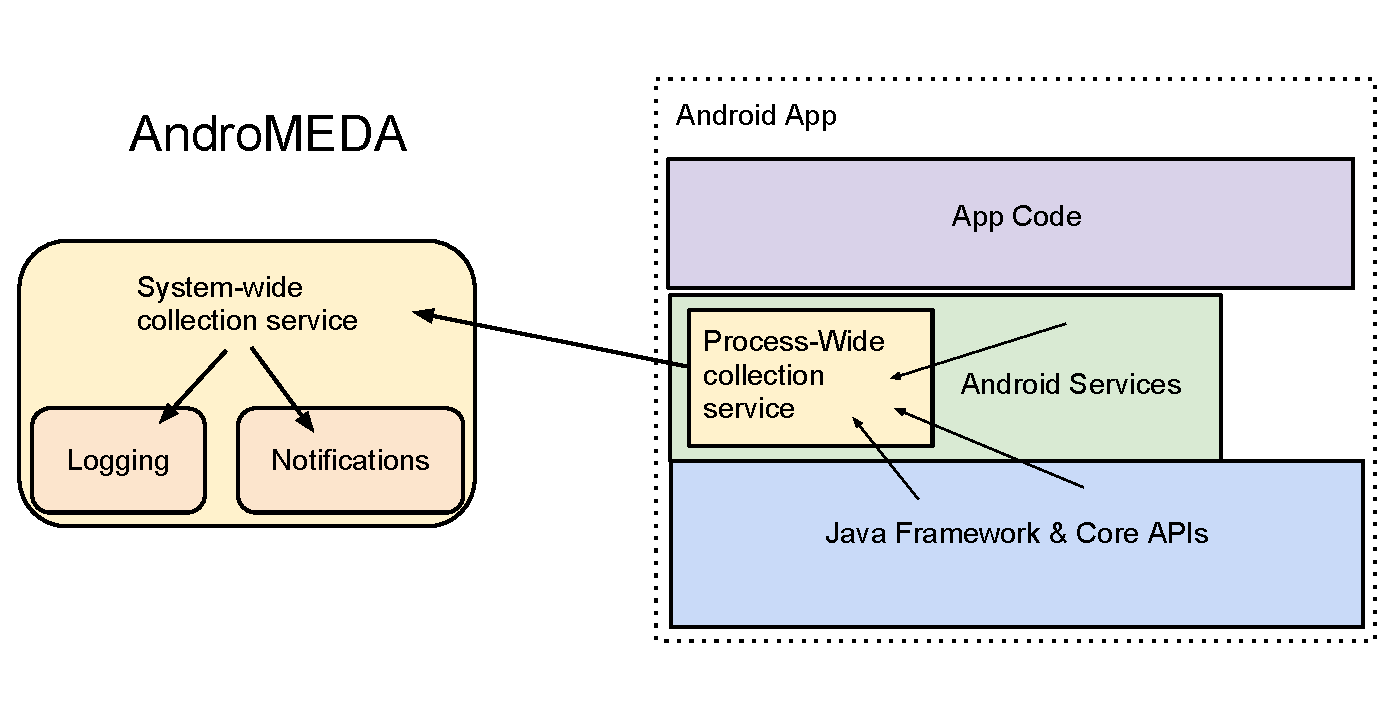
\includegraphics[width=1.0\columnwidth]{figs/AndroMEDA-Architecture-Overview}
\caption{AndroMEDA Architecture Overview}
\label{fig:andromedaoverview}
\end{center}
\end{figure}

The architecture, seen in Figure \ref{fig:andromedaoverview}, is organized into two main parts: A collection of hooks in the API, and a system service to collect this information. The collection of hooks in the API calls into a process-wide service that translates them into events that get sent to the global system service. At the start of every new Dalvik process, the process-wide collector installs hooks into the framework that notifies the collector when the APIs are called.

\begin{figure}[t]
\begin{center}
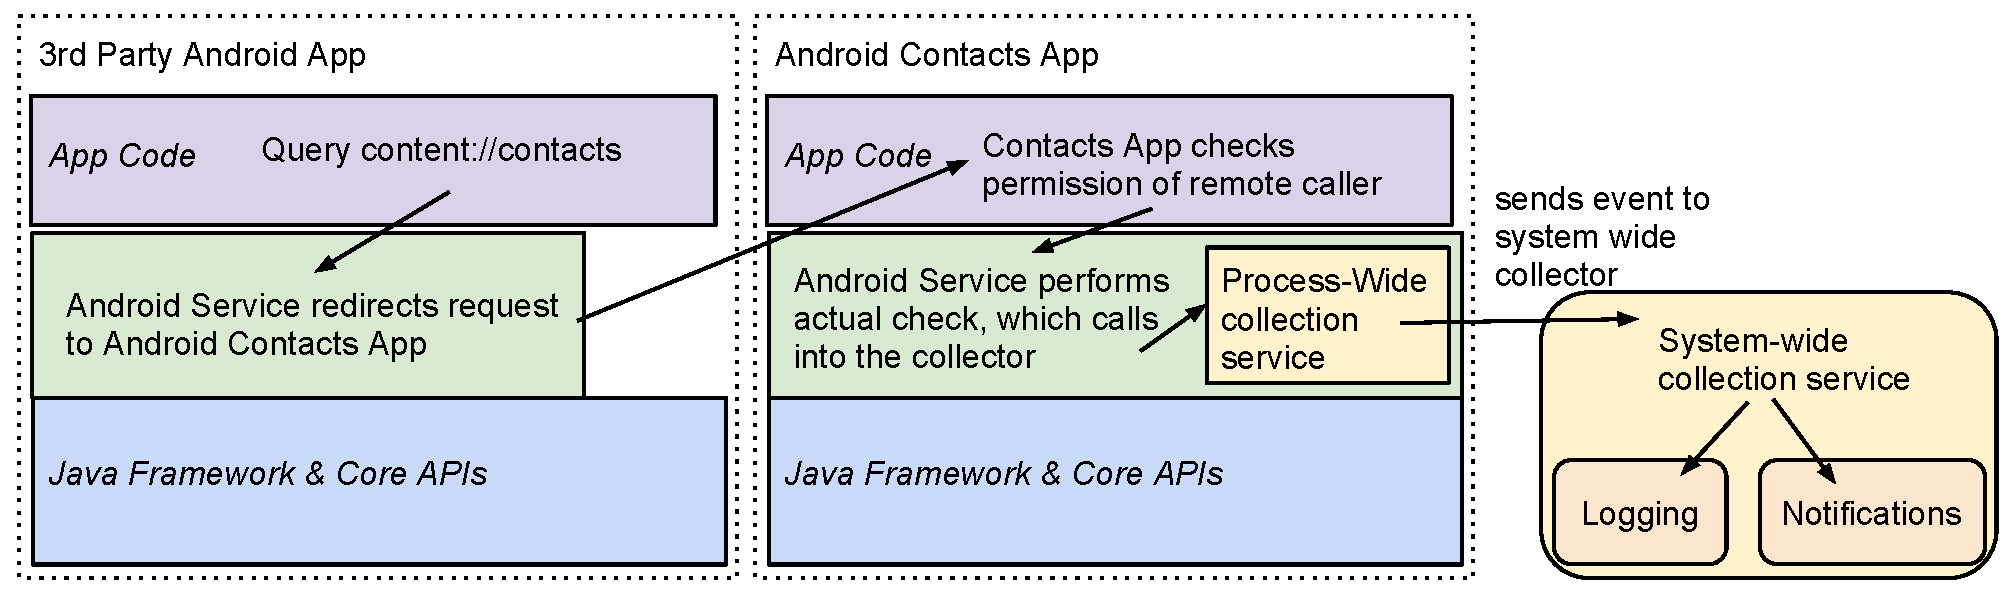
\includegraphics[width=1.0\columnwidth]{figs/AndroMEDA-Inter-App-Example}
\caption{Example code path of an app requesting data from the Contacts app}
\label{fig:interapp-example}
\end{center}
\end{figure}

The hooking mechanisms vary depending on the exact call being instrumented. Android has a standard mechanism for checking permissions in many cases, and we placed a hook where this is enforced. Usually, this takes place during an Remote Procedure Call (RPC) with the process that owns the data - and such, the remote UID is sent along, as seen in Figure \ref{fig:interapp-example}. Unfortunately many permissions are not checked through this manner, but Android Permissions Demystified\citep{felt2011android} has a comprehensive list of API calls and the permissions they require, making it easy to locate essential APIs to instrument. For the more difficult APIs, a static global callback variable is placed in every class we want to instrument. Upon launch of the process, our local collector populates these global variables with callbacks that marshal the data off to the main collection service. A quick null-check and then call are made to the callback at the appropriate times in the API's normal function, seen in Figure \ref{fig:camera-example}. Using this method, we are able to instrument any API call, getting more data than simply when the permission is checked.

\begin{figure}[t]
\begin{center}
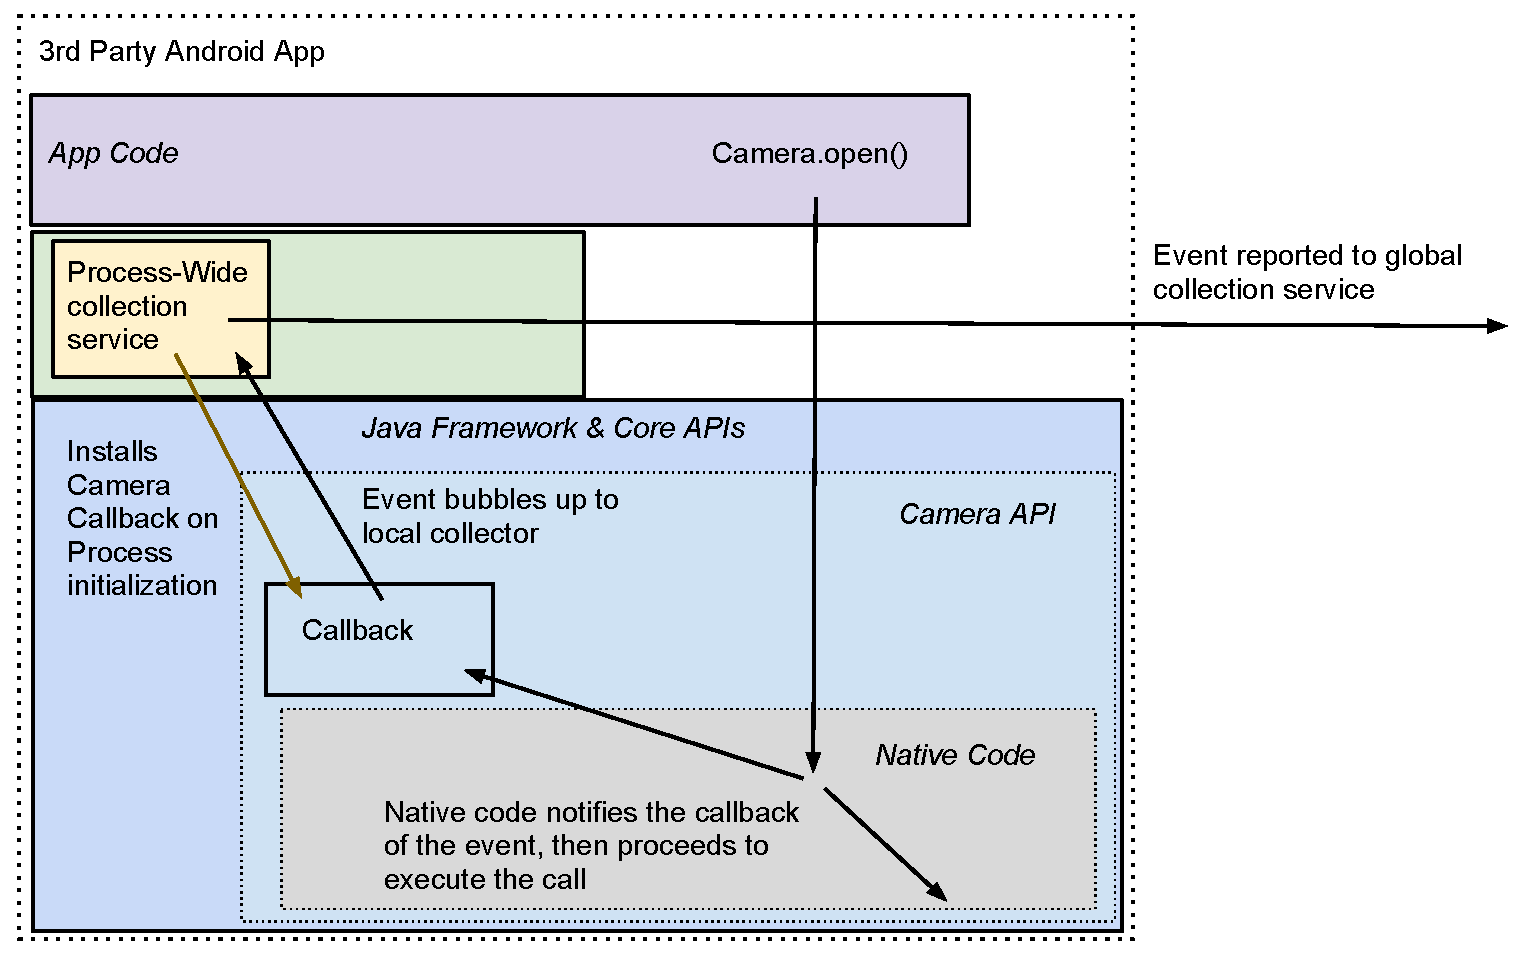
\includegraphics[width=1.0\columnwidth]{figs/AndroMEDA-Static-Example}
\caption{Example code path of instrumenting the Camera API}
\label{fig:camera-example}
\end{center}
\end{figure}

For c and c++ level code, we establish hooks in the Java Native Interface (JNI) - Java's method of communicating with native code - to call back to the main object, since using JNI to call back into Java from c is cumbersome and error prone, which then calls the process-wide callback accordingly, an example can be seen in Figure \ref{fig:camera-example}.

The ability to log virtually any API call is extremely valuable. Not only are permission events logged, but more fine grained events like the starting and stopping of an audio recording can be measured. Internet sockets are logged, along with all POST data set out. Not only is this system light-weight and fast, but it does so with as little modifications as possible. No kernel-level or dalvik-vm-level changes were required.

The global service serves as the central point of collection of all events. It runs in it's own process, and uses Binders (Android's RPC) to communicate with other processes, which feed events into it. These calls are asynchronous, and do not block the remote caller. The service is responsible for logging and processing the events, and taking action on them.

Two way communication is also possible. An app's local collector can query the global service and acquire a list of events for a given package, among other things. This allows user-level apps to be written to leverage AndroMEDAs findings.

\section{Companion App}
A companion app was written, to allow the user to inspect the information being gathered by AndroMEDA. The companion app responds to the Intents broadcast by the notifications that AndroMEDA displays to the user. This brings up a history of events logged by that app, and allows the user to take action. The user may report an app, or uninstall it. A simple web service was set up to aggregate these reports.

The companion app is significant because it does not require the AndroMEDA framework to be present on the phone to function. Despite no local logs being available, the companion app can still query the web service, and view event histories that other users have published.
